\documentclass[11pt,a4paper]{report}

\usepackage[hidelinks]{hyperref}
\usepackage[english]{babel}
\usepackage[svgnames]{xcolor}
\usepackage{graphicx}
\usepackage{minted}
\usepackage{multirow}

\begin{document}
\title{\textsc{Scarlet} \\ \large An OpenGL renderer implementing screen space reflection in a metallic workflow deferred rendering pipeline}
\author{Dario Ostuni}
\date{}
\maketitle

\tableofcontents

\chapter{Introduction}
\textit{Screen Space Reflection} (SSR) is a post-processing technique to calculate reflections using screen-space data. SSR is quite expensive in terms of computational resources needed (especially time resources), but when used in adequate situations it can create great reflections effects that could only be otherwise created with other, more expensive, global illumination techniques.

\textsc{Scarlet} is an OpenGL renderer that was written to show the implementations details and the pros and cons of the SSR technique. \textsc{Scarlet} is written in Rust and it implements SSR inside a metallic workflow deferred rendering pipeline. It will be shown how \textsc{Scarlet} functions, what are its main components, and how SSR is implemented inside it.

Using a benchmark scene the performance cost of SSR in various configurations and the quality of the effects it creates will be evaluated. In order to provide a more accurate evaluation \textsc{Scarlet} implements more than just the bare minimum graphics tooling needed for SSR, such as generic scene loading through glTF (GL Transmission Format), scene graph based rigid body animations, albedo textures support, gamma correction, etc.

\chapter{Scarlet}
\textsc{Scarlet} is a real-time renderer written in Rust. It can use either OpenGL ES 3.0 or OpenGL 3.3 with the \texttt{GL\_ARB\_ES3\_compatibility} extension as back-ends. It implements various utilities:
\begin{itemize}
	\item a window management layer (\texttt{Application}) that simplifies window creation (using \textit{winit}), context management (using \textit{glutin}) and OpenGL functions loading (using \textit{glad});
	\item an OpenGL debugging utility based on \texttt{GL\_KHR\_debug} (using \textit{log});
	\item a scene graph (\texttt{Scene}) that maintains the hierarchy of a scene using similarities (using \textit{nalgebra}) for describing parent-child transformations;
	\item a shader class (\texttt{Shader}) for easier shader management;
	\item a generic scene loader (\texttt{import\_scene} and related classes) that reads a scene in glTF format (using \textit{it}) and imports the scene graph, meshes, lights, cameras, rigid-body animations and albedo textures;
	\item a \textit{physically based rendering} algorithm called \textit{metallic workflow};
	\item a \textit{deferred rendering} pipeline, capable of showing the individual \textit{G-Buffers};
	\item a \textit{screen space reflection} post-processing shader based on \textit{binary cone-tracing};
	\item a \textbf{static\_viewer} tool to show a scene imported from a glTF file;
	\item an \textbf{exporter} tool to create a video from a scene animation;
	\item a \textbf{bench} tool to benchmark a scene.
\end{itemize}

\section{Application management}
The \texttt{Application} class is the entry point of \textsc{Scarlet}, its constructor takes an \texttt{ApplicationOptions} struct, which defines with which options the application will be built. \texttt{ApplicationOptions} has the following members:
\begin{itemize}
	\item \textbf{title}: the window title;
	\item \textbf{fullscreen}: a boolean flag for requesting a fullscreen window;
	\item \textbf{vsync}: a boolean flag for requesting vertical sync;
	\item \textbf{width}: the width of the window;
	\item \textbf{height}: the height of the window;
	\item \textbf{fps}: the maximum frames rendered per second;
	\item \textbf{debug\_gl}: a boolean flag to enable internal OpenGL debugging.
\end{itemize}

If not given a specific value, each of this options as a default value, which, for some, can be overridden using an environment variable:
\begin{itemize}
	\item \texttt{SCARLET\_FULLSCREEN}: boolean flag for \textbf{fullscreen};
	\item \texttt{SCARLET\_VSYNC}: boolean flag for \textbf{vsync};
	\item \texttt{SCARLET\_FPS}: floating-point number for \textbf{fps};
	\item \texttt{SCARLET\_DEBUG\_GL}: boolean flag for \textbf{debug\_gl}.
\end{itemize}

When the constructor is called, a window corresponding to the options given will be built. When ready to start the rendering loop, a closure can be passed to the method \texttt{run}, which will be run each time a new frame must be shown or when the window receives an input. Once \texttt{run} is invoked, \textsc{Scarlet} will never give back control of the application flow, instead it will be controlled by the closure passed which has to return at each invocation an \texttt{ApplicationAction} back:
\begin{itemize}
	\item \textit{Refresh}: the closure has updated the frame, and the window must refresh its contents;
	\item \textit{Quit}: the program must be closed;
	\item \textit{Nothing}: the closure has not updated the frame, and can be called again when needed.
\end{itemize}

\section{OpenGL debugging}
Debugging programs that use OpenGL can be hard, so an extension called \texttt{GL\_KHR\_debug} has been made by the Khronos Group to ease the process.

If the \texttt{GL\_KHR\_debug} extension is supported by the OpenGL driver and if the user has enabled the \textbf{debug\_gl} options, \textsc{Scarlet} will create an information reporting callback using \texttt{GL\_KHR\_debug} on the OpenGL driver side and the \textit{log} crate to show to the user the logging of the OpenGL driver.

If the OpenGL driver will have any information to report (such as invalid function calls, performance issues, etc.) \textsc{Scarlet} will report them on the console with a color representing the appropriate severity level:
\begin{itemize}
	\item Trace: {\color{magenta}magenta}
	\item Debug: {\color{cyan}cyan}
	\item Info: {\color{DarkGreen}dark green}
	\item Warning: {\color{Gold}gold}
	\item Error: {\color{FireBrick}firebrick}
\end{itemize}

\section{Shader class}
The \texttt{Shader} class is a utility to handle the loading, compilation and use of vertex and fragment shaders.

One can create a new \texttt{Shader} object and \texttt{attach} new shader sources, and \texttt{compile} them when finished. To aid OpenGL debugging functionality one can specify names for debugging by using the specialized \texttt{attach\_with\_name} and \texttt{compile\_with\_name} methods.

When needed, the shader can be used by calling the \texttt{activate} method. The \texttt{Shader} class also provide the loading of shader uniform variables using the \texttt{uniform*} family of methods, such as \texttt{uniform1ui}, \texttt{uniformMat4f}, etc.

If anything fails, it will be reported to the user on the console, in a simplified form if the OpenGL debugging functionality is disabled or in full form otherwise.

\section{Scene Graph}
In order to ease the display and manipulation of non-trivial scenes, a scene graph has been implemented. The scene graph is represented by the objects of the \texttt{Scene} class, while the scene graph nodes are of type \texttt{SceneNode}.

The \texttt{Scene} object contains the root \texttt{SceneNode} and other useful information, such as the animations present in the scene, performance information, the shaders used in the scene, etc. It also contains all the buffers needed for the deferred rendering pipeline.

A \texttt{SceneNode} represents a node in the scene graph, and it holds the following information:
\begin{itemize}
	\item \textbf{id}: a unique identifier;
	\item \textbf{transform}: the affine transformation relative to the parent, it's saved as a similarity (a scalar for the scale factor, an unit quaternion for the rotation and a vector for the translation);
	\item \textbf{children}: the children of this \texttt{SceneNode};
	\item \textbf{parent}: the parent of this \texttt{SceneNode};
	\item \textbf{name} (\textit{optional}): the name of this \texttt{SceneNode};
	\item \textbf{camera} (\textit{optional}): the \texttt{Camera} information of this node;
	\item \textbf{light} (\textit{optional}): the \texttt{Light} information of this node;
	\item \textbf{mesh} (\textit{optional}): the \texttt{Mesh} information of this node;
\end{itemize}

A \texttt{Camera} object represents a camera, and holds the perspective transformation (explicitly) and the position, look at, and up vector of the camera (implicitly, it's defined by composition of the transformations of the ancestor of the camera node).

A \texttt{Light} object represents a point or directional light, and holds the color, intensity and type of the light.

A \texttt{Mesh} object represents a mesh, which is a collection of geometric primitives (usually triangles) with properties such as position, normal vector, texture coordinates, etc. It also holds the information about the \texttt{Material} of the mesh, which is defined by an albedo color (possibly a texture), a metalness factor and a roughness factor.

When the scene needs to be rendered, the scene graph is traversed using an iterative depth-first search, accumulating the transformations during the path taken (applying also animations, if any), and all meshes are rendered, all lights are acknowledged and the perspective matrix is taken from the camera.

\section{glTF importer}
\textsc{Scarlet} uses glTF 2.0 as the scene input format. glTF is a complete and compact format for saving scenes which include a scene graph, meshes, textures, animations (rigid-body, skeletal or morphing), materials (metalness-roughness or specularity-glossiness), lights, cameras and much more. \textsc{Scarlet} only supports a subset of glTF.

\texttt{Scarlet} uses the \textit{gltf} crate to parse both serialized formats of glTF (\texttt{.gltf} and \texttt{.glb}) and decode the textures contained within. When parsed, it construct a \texttt{Scene} by walking the glTF scene graph and converting it to the \textsc{Scarlet} internal scene graph format, while also creating all the necessary OpenGL vertex buffer objects, vertex array objects and textures.

\section{Metallic Workflow}
\textit{Physically Based Rendering} (PBR) is a series of techniques to render realistic looking scenes. What it differs from other approaches as \textit{Gouraud} and \textit{Phong} is that PBR tries to be based on how light actually works in real life.

\textit{Metallic Workflow} is one such PBR technique, originally developed by Disney and then adapted to work in real-time by Epic Games. When using \textit{Metallic Workflow} to each material is assigned an albedo color, a metalness factor and a roughness factor.

The whole rendering process can be described by the following formula:
$$ L_o(p, \omega_o) = \int \limits_{\Omega} k_d \frac{c}{\pi} + \frac{DFG}{4(\omega_o \cdot n)(\omega_i \cdot n)} L_i(p, \omega_i)n \cdot \omega_i d \omega_i $$

where:
\begin{itemize}
	\item $L_o(p, \omega_o)$ is a function indicating how much light is going in direction $\omega_o$ from point $p$;
	\item $k_d \frac{c}{\pi} + \frac{DFG}{4(\omega_o \cdot n)(\omega_i \cdot n)}$ is the Cook--Torrance Bidirectional Reflective Distribution Function, in other words, given an incoming direction $\omega_i$, an outgoing direction $\omega_o$ and a surface normal $n$ it gives the contribution of the light coming from $\omega_i$ to the direction $\omega_o$;
	\item $k_d \frac{c}{\pi}$ is the Lambertian diffuse part of Cook--Torrance BRDF, where $k_d$ is the fraction of the light that gets refracted and $c$ is the surface color;
	\item $D$ is the \textit{normal distribution function}, which measures how much the surface normals are aligned with the halfway vector (the normalized sum of the light direction and view direction); it's calculated as $\frac{\alpha^2}{\pi((n \cdot h)^2(\alpha^2 - 1) + 1)^2}$ where $\alpha$ is the roughness factor, $h$ is the halfway vector and $n$ is the surface normal;
	\item $F$ is the \textit{Fresnel equation}, which is the ratio of the light which gets reflected over the light that gets refracted according to the angle we're looking at a surface; it's calculated as $F_0 + (1 - F_0)(1 - h \cdot v)^5$ where $v$ is the view direction and $F_0$ is the reflectivity of the surface, which is approximated by the product of the metalness factor and the surface color;
	\item $G$ is the \textit{geometry function}, which measures how much the surface overshadows itself; it's calculated as $\frac{n \cdot v}{(n \cdot v)(1 - \frac{(\alpha + 1)^2}{8}) + \frac{(\alpha + 1)^2}{8}}$;
	\item $L_i(p, \omega_i)$ is a function indicating how much light is incoming from direction $\omega_i$ to point $p$;
	\item $n \cdot \omega_i$ scales the incoming light energy from $\omega_i$ using the angle between $\omega_i$ and $n$;
	\item $\int \limits_{\Omega} ~\dots~ d \omega_i$ is a surface integral, meaning that it's the sum of the contribution of each incoming direction $\omega_i$.
\end{itemize}

\section{Deferred rendering}
\textit{Deferred rendering} is a technique used to \textit{defer} as much as possible the heavy computations such as lighting, in order to reduce the number of geometric primitives on which the heavy computation will be run.

In order to do so a first \textit{geometry pass} is performed, where certain information (such as fragment positions, normals, etc.) are saved in some special framebuffers called \textit{G-buffer}s. One all vertices have been processed, only the visible fragments will remain in the \textit{G-buffer}s, and we can use the information collected in them to then do the lighting, thus only doing the heavy computations for only what will actually be displayed.

\textsc{Scarlet} implements a multi-pass deferred rendering pipeline, in which the passes are:
\begin{enumerate}
	\item geometry pass: renders the scene and collects information in \textit{G-buffer}s about position~[\ref{deferred:position}], normals~[\ref{deferred:normal}], albedo~[\ref{deferred:albedo}], metalness~[\ref{deferred:metalness}], roughness~[\ref{deferred:roughness}] and depth~[\ref{deferred:depth}];
	\item PBR pass: using the information collected from the geometry pass, metallic workflow is applied to produce a PBR shading of the scene~[\ref{deferred:pbr}];
	\item SSR pass: reflections are calculated for all points using screen space reflections~[\ref{deferred:ssr}];
	\item final pass: the frames produced from the PBR and SSR passes are merged to produce the final rendered image~[\ref{deferred:final}].
\end{enumerate}

\begin{figure}[htp]
	\centering
	\includegraphics[width=\textwidth]{deferred/00position.png}
	\caption{Position \textit{G-buffer}}
	\label{deferred:position}
\end{figure}

\begin{figure}[htp]
	\centering
	\includegraphics[width=\textwidth]{deferred/01normal.png}
	\caption{Normal \textit{G-buffer}}
	\label{deferred:normal}
\end{figure}

\begin{figure}[htp]
	\centering
	\includegraphics[width=\textwidth]{deferred/02albedo.png}
	\caption{Albedo \textit{G-buffer}}
	\label{deferred:albedo}
\end{figure}

\begin{figure}[htp]
	\centering
	\includegraphics[width=\textwidth]{deferred/03metalness.png}
	\caption{Metalness \textit{G-buffer}}
	\label{deferred:metalness}
\end{figure}

\begin{figure}[htp]
	\centering
	\includegraphics[width=\textwidth]{deferred/04roughness.png}
	\caption{Roughness \textit{G-buffer}}
	\label{deferred:roughness}
\end{figure}

\begin{figure}[htp]
	\centering
	\includegraphics[width=\textwidth]{deferred/05depth.png}
	\caption{Depth \textit{G-buffer}}
	\label{deferred:depth}
\end{figure}

\begin{figure}[htp]
	\centering
	\includegraphics[width=\textwidth]{deferred/06pbr.png}
	\caption{PBR \textit{G-buffer}}
	\label{deferred:pbr}
\end{figure}

\begin{figure}[htp]
	\centering
	\includegraphics[width=\textwidth]{deferred/07ssr.png}
	\caption{SSR \textit{G-buffer}}
	\label{deferred:ssr}
\end{figure}

\begin{figure}[htp]
	\centering
	\includegraphics[width=\textwidth]{deferred/08final.png}
	\caption{Final \textit{G-buffer}}
	\label{deferred:final}
\end{figure}

\section{Screen Space Reflection}
\textit{Screen Space Reflection} (SSR) is a technique to reuse already calculated information about the scene to compute reflections. In \textsc{Scarlet} SSR uses the position, normal, metalness, roughness, depth and PBR \textit{G-Buffer}s.

The idea behind SSR is to calculate, for each point, the reflection direction using the view direction and the surface normal of that point, and do some kind of ray-tracing in the reflected direction to find the point that will be reflected there, using the depth buffer for testing for collisions.

\textsc{Scarlet} implements a variation of \textit{binary cone-tracing}, which consists of a four phases algorithm to determine which point will be reflected. Once the point will be found il will be sampled using a bicubic interpolation filter and saved in the SSR \textit{G-Buffer}. The algorithm has been designed to always end in a fixed amount of time (controlled by a \texttt{MAX\_ITERATIONS} parameter), in order to being tunable to guarantee some minimum FPS.

\subsection{Phase 1: finding a collision}
The first phase tries to find if the reflected ray collides with something within the view-space unit cube or not. It does so by applying a technique called \textit{binary exponentiation}: it starts with a small $\delta$ and advances the ray of this $\delta$ in the ray direction; it checks for intersection: if it does intersect, this phase finishes, otherwise it repeats the process up to \texttt{MAX\_ITERATIONS} times doubling $\delta$ each time. If at some point the ray goes outside the unit cube, it resets its position to the previous one and resets $\delta$ to its initial value. The implementation used in \textsc{Scarlet} can be found in listing \ref{ssr:phase1}.

\begin{listing}
	\inputminted[tabsize=2, frame=lines,
framesep=2mm,
baselinestretch=1.2,
bgcolor=LightGray,
fontsize=\footnotesize,
linenos]{glsl}{code/phase1.frag}
	\caption{SSR - Phase 1}
	\label{ssr:phase1}
\end{listing}

\subsection{Phase 2: checking missing geometry}
Once the previous phase has found an intersection point with the geometry, this phase checks if there is some object that is nearer to the viewer that needs to be reflected. To check this, the space between the intersection point and the point we're calculating the reflection is partitioned in \texttt{MAX\_ITERATIONS} chunks, and each of the is tested for intersection. The nearest that tests positive for intersection will be selected as this phase output. Code for this phase can be found in listing \ref{ssr:phase2}.

\begin{listing}
	\inputminted[tabsize=2, frame=lines,
framesep=2mm,
baselinestretch=1.2,
bgcolor=LightGray,
fontsize=\footnotesize,
linenos]{glsl}{code/phase2.frag}
	\caption{SSR - Phase 2}
	\label{ssr:phase2}
\end{listing}

\subsection{Phase 3: binary searching the bound}
At this point we have the starting point and one other point that we know intersects with some object, at this point, since there is an high probability that the functions that tells us if there is an intersection at some point between these two points is convex, we can binary search (allowing up to \texttt{MAX\_ITERATIONS} iterations to gain precision) where is the nearest point that intersects. We will output this point for the input of the next phase. Code for this phase can be found in listing \ref{ssr:phase3}.

\begin{listing}
	\inputminted[tabsize=2, frame=lines,
framesep=2mm,
baselinestretch=1.2,
bgcolor=LightGray,
fontsize=\footnotesize,
linenos]{glsl}{code/phase3.frag}
	\caption{SSR - Phase 3}
	\label{ssr:phase3}
\end{listing}

\subsection{Phase 4: fine-grained backtracking}
In the final phase we want to check if we missed some fine detail of the object that might be non-convex. To do this, we start from the point found in the last phase and backtrack using steps of the initial $\delta$ size, up to \texttt{MAX\_ITERATIONS} times. If there is an intersection with something, we'll output the last point that tested positive, otherwise we'll output the input point. Code for this phase can be found in listing \ref{ssr:phase4}.

\begin{listing}
	\inputminted[tabsize=2, frame=lines,
framesep=2mm,
baselinestretch=1.2,
bgcolor=LightGray,
fontsize=\footnotesize,
linenos]{glsl}{code/phase4.frag}
	\caption{SSR - Phase 4}
	\label{ssr:phase4}
\end{listing}

\section{Static viewer}
To import and see a, optionally animated, scene with \textsc{Scarlet} using the \textit{static viewer} tool. In order to build the tool the command to issue is:
\begin{minted}{console}
$ cargo build --release --example static_viewer
\end{minted}
This will build the \textsc{Scarlet} scene viewer, that can then be used to import and see a scene by passing it as a CLI argument, for example by issuing:
\begin{minted}{console}
$ cargo run --release --example static_viewer scene/room.glb
\end{minted}
When the program is opened it will show the scene until closed, and if there is an animation il will loop indefinitely. By default the final rendered frame is shown, but by using the left and right arrows on the keyboard different \textit{G-Buffer}s will be shown.
\section{Video exporter}
The \textit{video exporter} tool has been created to aid the creation of videos from scene animations. The CLI works in the same way as the viewer, but when run it will output the frames in PNG format.

An example of usage:
\begin{minted}{console}
$ cargo build --release --example exporter
$ cargo run --release --example exporter scene/room_animated.glb
\end{minted}

\section{Benchmark tool}
The \textit{benchmark} tool has been created to benchmark the performance of \textsc{Scarlet} on an animated scene. It will render the animated scene and at regular intervals it will record the current FPS. At the end it will create a file called \texttt{benchmark.json} containing the information collected.

An example of usage:
\begin{minted}{console}
$ cargo build --release --example bench
$ cargo run --release --example bench scene/room_animated.glb
\end{minted}

\chapter{Evaluation}
In order to evaluate the performance of \textsc{Scarlet} at various levels of SSR precision, a benchmark scene has been created, called \textsc{Scarlet--Room}.

\begin{figure}[htp]
	\centering
	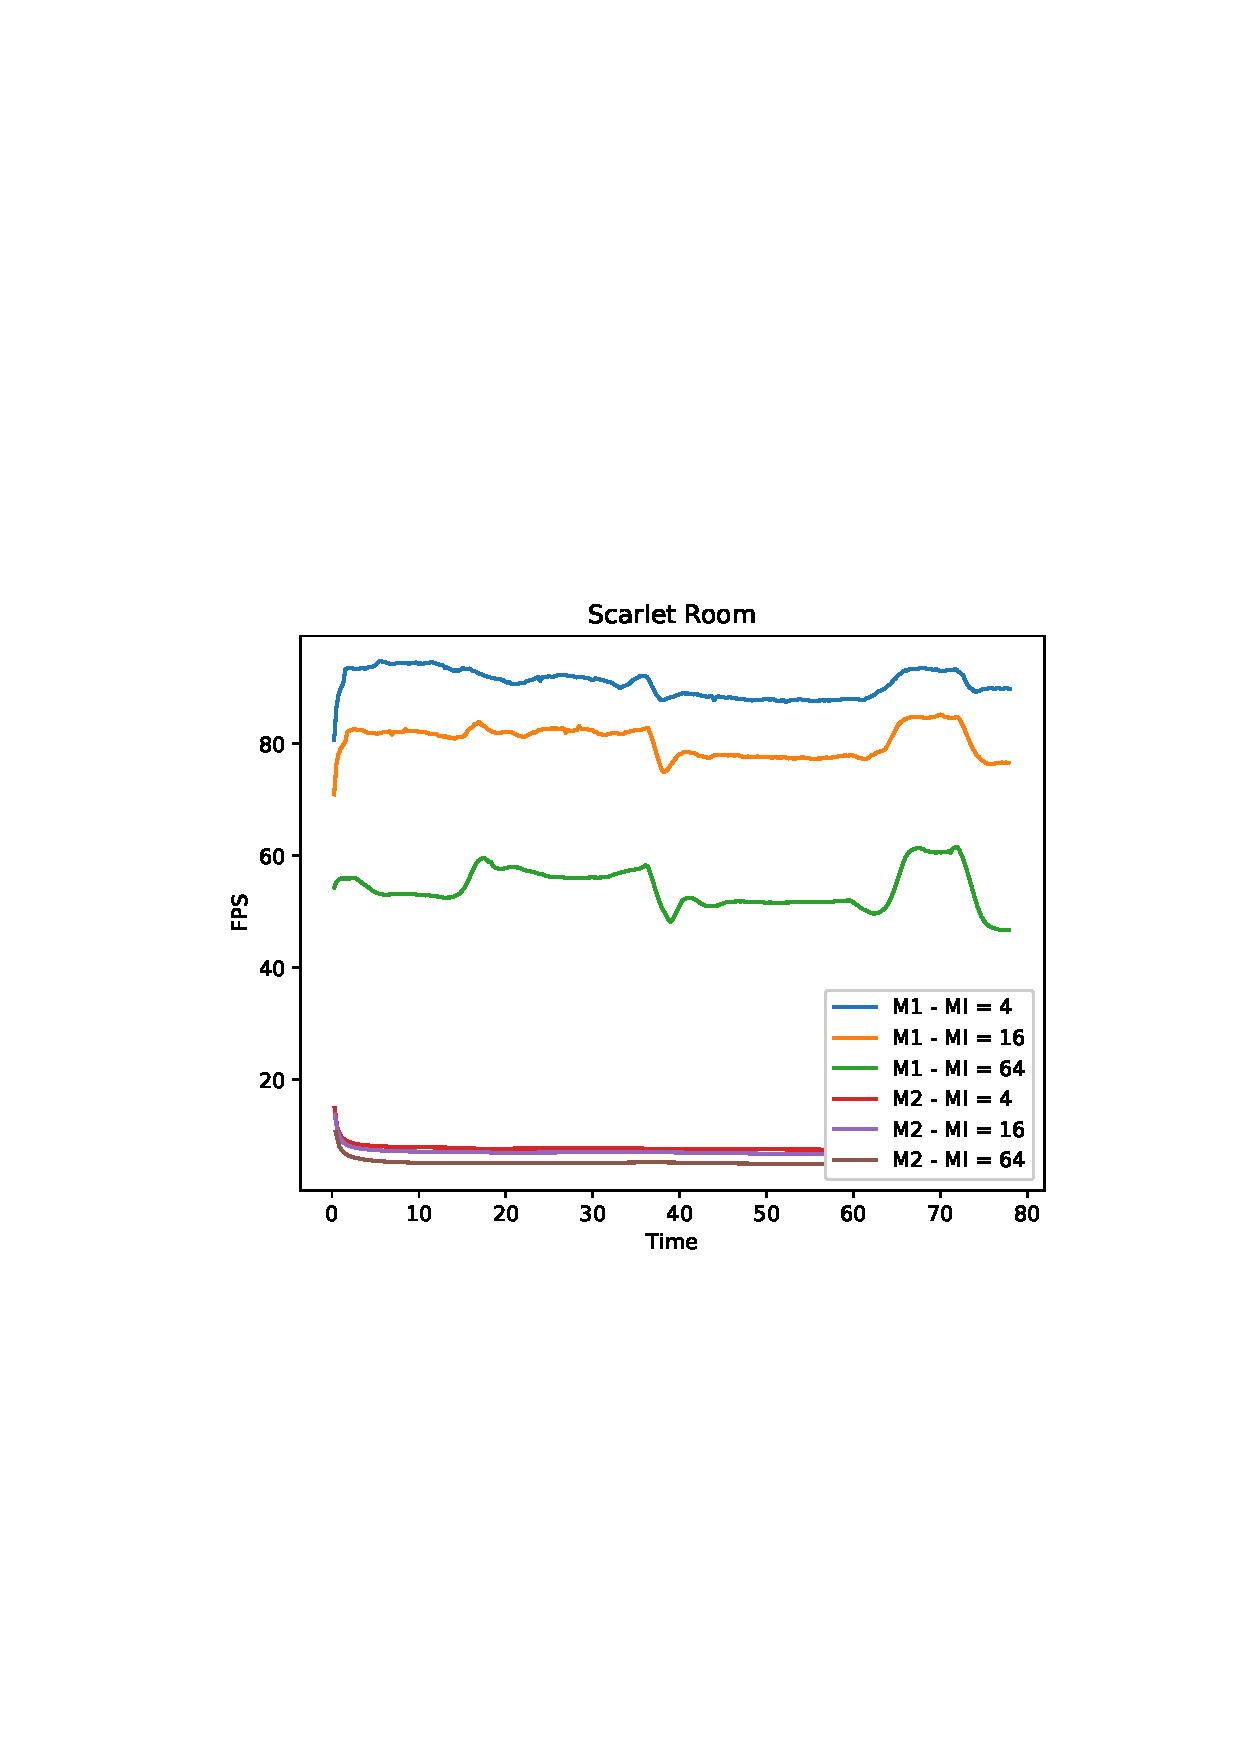
\includegraphics[width=\textwidth]{benchmark/benchmark.png}
	\caption{A frame from \textsc{Scarlet--Room} benchmark}
	\label{eval:example}
\end{figure}

The benchmark has been designed to highlight specific features of \textsc{Scarlet}, including: scene graph animations, deferred rendering and screen space reflection. To give an evaluation of the performance and the quality of SSR, the benchmark has been run on two machines varying the SSR quality parameter \texttt{MAX\_ITERATIONS}. The machines used to run the benchmark are:

\begin{center}
	\begin{tabular}{ | c | c | c | c | } \hline
		Name & CPU & RAM & GPU \\ \hline
		M1 & Intel 6700K & 64 GiB DDR4 2133 MHz & NVIDIA GTX 980M \\
		M2 & Intel 7100U & 20 GiB DDR4 2133 MHz & Intel HD Graphics 620 \\
		\hline \end{tabular}
\end{center}

The benchmark has been run using the same resolution on all machines, which is $1920 \times 1080$. The benchmark has been run multiple times varying the \texttt{MAX\_ITERATIONS} parameter to the values $4$, $16$ and $64$.

\begin{figure}[htp]
	\centering
	\includegraphics[width=\textwidth]{benchmark/4.png}
	\caption{A frame from \textsc{Scarlet--Room} with $\texttt{MAX\_ITERATIONS} = 4$}
	\label{eval:4}
\end{figure}

\begin{figure}[htp]
	\centering
	\includegraphics[width=\textwidth]{benchmark/16.png}
	\caption{A frame from \textsc{Scarlet--Room} with $\texttt{MAX\_ITERATIONS} = 16$}
	\label{eval:16}
\end{figure}

\begin{figure}[htp]
	\centering
	\includegraphics[width=\textwidth]{benchmark/64.png}
	\caption{A frame from \textsc{Scarlet--Room} with $\texttt{MAX\_ITERATIONS} = 64$}
	\label{eval:64}
\end{figure}

As shown in figures \ref{eval:4}, \ref{eval:16} and \ref{eval:64} varying the \texttt{MAX\_ITERATIONS} parameter produces very different results regarding the precision of reflections. A full pre-rendered video of the benchmark can be found on YouTube at \url{https://www.youtube.com/watch?v=wf36zKOmeuM}. This video can be used to gain an insight of how the benchmark looks like. It has been rendered at resolution $3840 \times 2160$, 60 frames per second, with $\texttt{MAX\_ITERATIONS} = 64$.

We can predict that producing the higher quality images, obtained by setting an higher value of \texttt{MAX\_ITERATIONS}, will likely have an impact on performance. The benchmark results will show how much of an impact there is:

\begin{center}
	\begin{tabular}{|c|c|c|c|c|}
		\hline
		\textbf{Machine}    & \textbf{\texttt{MAX\_ITERATIONS}} & \textbf{Avg. FPS} & \textbf{Min. FPS} & \textbf{Max. FPS} \\ \hline
		\multirow{3}{*}{M1} & 4                                 & 90.77             & 80.69             & 94.73             \\
		& 16                                & 80.41             & 70.95             & 85.21             \\
		& 64                                & 54.20             & 46.77             & 61.53             \\ \hline
		\multirow{3}{*}{M2} & 4                                 & \phantom{0}7.79   & \phantom{0}7.52   & 14.98             \\
		& 16                                & \phantom{0}7.05   & \phantom{0}6.69   & 13.76             \\
		& 64                                & \phantom{0}5.16   & \phantom{0}4.75   & 10.69             \\ \hline
	\end{tabular}
\end{center}

\section{Results}

\begin{figure}[htp]
	\centering
	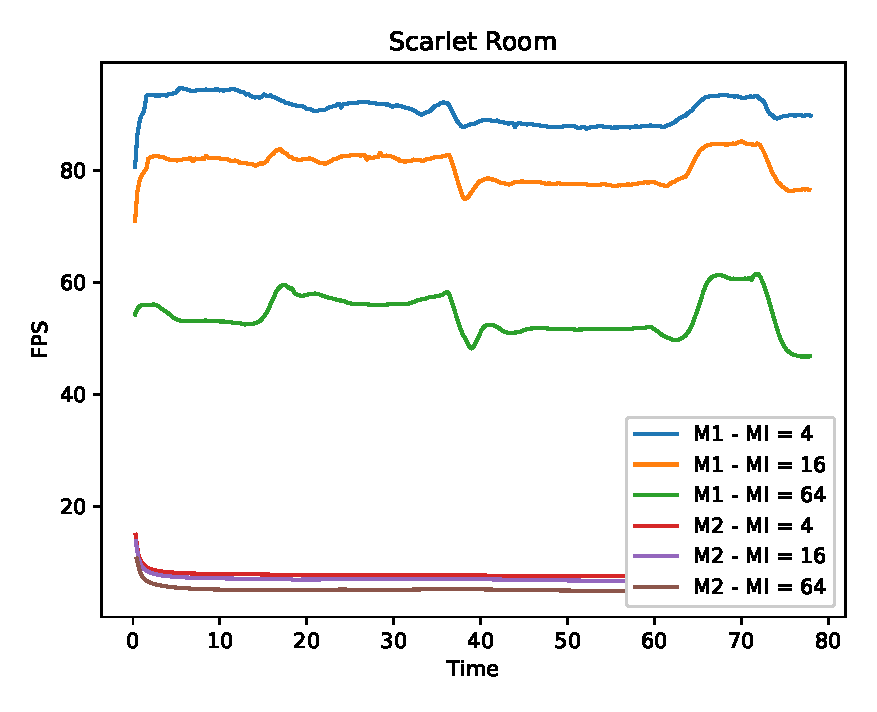
\includegraphics[width=\textwidth]{benchmark/benchmark.eps}
	\caption{Benchmark results}
	\label{eval:graph}
\end{figure}



\end{document}
